\documentclass[aspectratio=169]{beamer}

\usetheme{NRLpresentationGWU}
\usepackage{NRLcolors}

%\titlegraphic{\includegraphics[width=0.9\textwidth]{$HOME/Documents/TAVEX/gmt/TAVEX-overview-3}}% optional

\setbeamerfont{footnote}{size=\tiny}
%\beamertemplatenavigationsymbolsempty


\usepackage[style=authortitle-comp,maxnames=1]{biblatex} % PGR: backend=biber???
\addbibresource{../References/PhD_refs.bib}

\usepackage{graphicx}
\graphicspath{{../Figures/}}

\usepackage{amsmath,amssymb,amsfonts}
\usepackage{upgreek}
\usepackage[retainorgcmds]{IEEEtrantools}

%\usepackage{hyperref}
%\usepackage[capitalize]{cleveref}

\usepackage{relsize}

\usepackage{bm}
\usepackage{hhline}


\setlength{\fboxsep}{3pt}
\setlength{\fboxrule}{2pt}


\usepackage{mathfont_shortcuts}
\usepackage{PhDmath}


\DeclareMathOperator{\nbarrm}{\bar{\mathrm{n}}}


\newcommand\independent{\protect\mathpalette{\protect\independenT}{\perp}}
\def\independenT#1#2{\mathrel{\rlap{$#1#2$}\mkern2mu{#1#2}}}




\title{Bayesian Learning for Regression using Dirichlet Prior Distributions of Varying Localization}
%\subtitle{Work Supported by the U.S. Office of Naval Research}% optional

\author[Rademacher \& Doroslova\v{c}ki]{Paul Rademacher\inst{1} \and Milo\v{s} Doroslova\v{c}ki\inst{2}}
\institute[NRL,~GWU] 
{
  \inst{1}
  U.S. Naval Research Laboratory\\Radar Division
  \and
  \inst{2}
  The George Washington University\\Department of Electrical and Computer Engineering
}


\date{July 11, 2021}


%\NRLcredit{Work Supported by the U.S. Office of Naval Research}% optional
%\NRLmark{FOR OFFICIAL USE ONLY}% optional
%\NRLpatents{Example Patents\\7,749,438 and 7,754,145}% optional

\NRLdist{DISTRIBUTION A. Approved for public release: distribution unlimited.}
%\NRLfoot{DISTRIBUTION A. Approved for public release: distribution unlimited.}


\begin{document}


\begin{frame}
\titlepage
\end{frame}


\section{Introduction} 

\begin{frame}
\frametitle{Bayesian Learning}
%\frametitle{Introduction}
%\framesubtitle{Part I}

Bayesian approaches to statistical learning attempt to make better decisions by exploiting \alert{prior knowledge} regarding the data-generating distribution:

\vspace{1em}

\begin{columns}[T]

\begin{column}{.5\linewidth}

\centering
\large \textbf{\underline{Informative}} \normalsize
\vspace{0.5em}
\begin{itemize}
\item If the prior is localized around the true data-generating model, low-risk decisions can be made even with limited training data
\item Priors that assign low weighting to the true model may not be able to realize satisfactory performance 
\end{itemize}


\end{column}

\vrule

\begin{column}{.5\linewidth}

\centering
\large \textbf{\underline{Non-Informative}} \normalsize
\vspace{0.5em}
\begin{itemize}
\item Learners designed with minimally localized priors respond strongly to training data, avoiding the drawbacks of misinformed prior knowledge
\item If the data volume is limited, high variance "overfit" solutions can occur
%\item Learners designed with approximately uniform priors will not perform as well as those made with well-selected informative priors
%\item Avoid high risk inherent to learners made by mismatched informative priors
\end{itemize}



\end{column}

\end{columns}

\end{frame}




\begin{frame}
\frametitle{The Dirichlet Prior}
%\frametitle{Introduction}
%\framesubtitle{Part II}

Dirichlet prior distributions have a number of desirable properties:
\begin{itemize}
%\item Often, priors are termed non-informative as long as they are approximately uniform over their \underline{limited support}. For example, a parametric regression function might use a high covariance Gaussian vector prior to characterize a subset of probability distributions
\vspace{0.5em}
\item \alert{Full support} over the space of data-generating distributions, guaranteeing \emph{consistent estimation} of the true data model
\vspace{0.5em}
\item They are \alert{conjugate priors} for independent, identically distributed observations \footfullcite{ferguson}, leading to \emph{closed-form} posterior distributions
\vspace{0.5em}
\item \alert{Flexible parameterization} enabling \emph{both} maximally and minimally informative priors and thus a wide range of learning solutions
\end{itemize}

\end{frame}



\section{Data Model and Regression Objective}


\begin{frame}
\frametitle{Data Representation}

\begin{description}
\item[Observable random variable:] $\xrm \in \Xcal \subset \Rbb$
\item[Unobservable random variable:] $\yrm \in \Ycal \subset \Rbb$
\item[Observable training data:] $\Drm \in \Dcal = \{\Ycal \times \Xcal\}^N$
\end{description}

\vspace{0.5em}

Independently, identically distributed according to an \underline{unknown} probability mass function (PMF) 
\begin{equation*}
\uptheta \in \Theta = \left\{ \theta \in {\Rbb_{\geq 0}}^{\Ycal \times \Xcal}: \sum_{y \in \Ycal} \sum_{x \in \Xcal} \theta(y,x) = 1 \right\} \ ,
\end{equation*}
such that $\Prm_{\yrm,\xrm | \uptheta}(y,x | \theta) = \Prm_{\Drm_n | \uptheta}(y,x | \theta) = \theta(y,x)$.

\hrulefill

\vspace{0.5em}
\textit{Alternate Notation}: $\uptheta \Leftrightarrow \big( \upthetam,\upthetac \big)$
\begin{itemize}
\item Marginal model $\upthetam \equiv \sum_{y \in \Ycal} \uptheta(y,\cdot) = \Prm_{\xrm | \uptheta}$ over the set $\Xcal$ 
\item Conditional models $\upthetac(x) \equiv \uptheta(\cdot,x) / \upthetam(x) = \Prm_{\yrm | \xrm,\uptheta}$ over the set $\Ycal$
\end{itemize}

\end{frame}




\begin{frame}
\frametitle{Sufficient Statistic}
\framesubtitle{Transform}

\begin{columns}[c]

\begin{column}{.5\linewidth}

Using the i.i.d. assumption,
\begin{IEEEeqnarray}{C}
\Prm_{\Drm | \uptheta}\big( D | \theta \big) = \left( \prod_{y \in \Ycal} \prod_{x \in \Xcal} \theta(y,x)^{\Psi(y,x;D)} \right)^N \nonumber 
\end{IEEEeqnarray}
where data is represented using $\Psi : \Dcal \mapsto \Uppsi \subset \Theta$, defined as
\begin{equation*}
\Psi(y,x;D) = N^{-1} \sum_{n=1}^N \delta \big[ (y,x),D_n \big] \;.
\end{equation*}
%and the range is
%\begin{equation*}
%\Uppsi = \left\{ \frac{n}{N} \in {\Zbb_{\geq 0}}^{\Ycal \times \Xcal}: \sum_{y \in \Ycal} \sum_{x \in \Xcal} n(y,x) = N \right\}
%\end{equation*}

\end{column}

\vrule
\hspace{0.5ex}
\begin{column}{.5\linewidth}

\begin{itemize}
\item Empirical distribution $\Psi(\Drm)$ is a \alert{sufficient statistic}\footnotemark ~for the model $\uptheta$
\vspace{0.5em}
\item Efficient: $|\Uppsi| = \binom{N+|\Ycal||\Xcal|-1}{|\Ycal||\Xcal|-1} \leq |\Dcal|$
\vspace{1.5em}
\item [$\Rightarrow$] \textbf{Represent data using new random process $\uppsi \equiv \Psi(\Drm) \in \Uppsi$}

%\vspace{0.5em}
%\item \textit{Alternate Notation}: $\uppsi \Leftrightarrow \big( \uppsim,\uppsic \big)$
%\begin{itemize}
%\item Marginal $\uppsim \equiv \sum_{y \in \Ycal} \uppsi(y,\cdot)$
%\item Conditional $\uppsic(\xrm) \equiv \uppsi(\cdot,\xrm) / \uppsim(x)$
%\end{itemize}
\end{itemize}

\end{column}

\end{columns}

\footcitetext{bernardo}
%\footcitetext{feller}

\end{frame}



\begin{frame}
\frametitle{Sufficient Statistic}
\framesubtitle{Distribution}

\begin{itemize}
\item Conditioned on the true model, the data statistic is an "Empirical" random process $\uppsi | \uptheta \sim \Emp(N,\uptheta)$
\begin{itemize}
\item Equivalent to a normalized multinomial random process \footfullcite{minka-multi}
\end{itemize}
\item As $N \to \infty$, the random process converges to $\uppsi | \uptheta \inprob \uptheta$
\begin{itemize}
\item [$\Rightarrow$] Enables \alert{consistent} estimation of model
\end{itemize}

\end{itemize}



\hrulefill

\begin{columns}[c]

\begin{column}{.5\linewidth}
\textit{Alternate Notation}: $\uppsi \Leftrightarrow \big( \uppsim,\uppsic \big)$
\begin{itemize}
\item Marginal $\uppsim \equiv \sum_{y \in \Ycal} \uppsi(y,\cdot)$
\item Conditional $\uppsic(x) \equiv \uppsi(\cdot,x) / \uppsim(x)$
\end{itemize}
\end{column}

\begin{column}{.5\linewidth}
By the aggregation property \footnotemark,
\begin{itemize}
\item $\uppsim | \upthetam \sim \Emp(N,\upthetam)$
\item $\uppsic(x) | \uppsim(x),\upthetac(x) \sim \Emp\big( N \uppsim(x),\upthetac(x) \big)$ are independent
\end{itemize}
\end{column}

\end{columns}

\footcitetext{johnson}

\end{frame}



\begin{frame}
\frametitle{Objective}

\begin{itemize}
\item Design a regression function $f: \Uppsi \mapsto \Rbb^{\Xcal}$ to minimize the expected squared-error with respect to $\uptheta$:
\begin{IEEEeqnarray}{rCl} \label{eq:risk_cond_SE}
\Rcal_{\Theta}(f ; \uptheta) = \Erm_{\yrm,\xrm,\uppsi | \uptheta} \Big[ \big( f(\xrm;\uppsi)-\yrm \big)^2 \Big] & \equiv & \underbrace{\Erm_{\xrm | \upthetam} \left[ \Sigma_{\yrm | \xrm,\upthetac} \right]}_{\mathlarger{\Rcal_{\Theta}^*(\uptheta)}} + \underbrace{\Erm_{\xrm,\uppsi | \uptheta} \Big[ \big( f(\xrm;\uppsi) - \mu_{\yrm | \xrm,\upthetac} \big)^2 \Big]}_{\mathlarger{\Rcal_{\Theta, \mathrm{ex}}(f ; \uptheta)}} \nonumber
\end{IEEEeqnarray}

\item Clairvoyant \footfullcite{kay-det} regressor $f_{\Theta}(\xrm;\upthetac) = \mu_{\yrm | \xrm,\upthetac}$ achieves irreducible squared-error $\Rcal_{\Theta}^*(\uptheta)$

\item Excess squared-error can be decomposed into \alert{bias} and \alert{variance} terms:
\begin{IEEEeqnarray}{rCl} \label{eq:risk_cond_ex_SE}
\Rcal_{\Theta, \mathrm{ex}}(f ; \uptheta) & \equiv & \Erm_{\xrm | \upthetam} \left[ \Big( \Erm_{\uppsi | \uptheta}\big[ f(\xrm;\uppsi) \big] - f_{\Theta}(\xrm;\upthetac) \Big)^2 + \Crm_{\uppsi | \uptheta}\big[ f(\xrm;\uppsi) \big] \right] \nonumber 
\end{IEEEeqnarray}

\end{itemize}

\end{frame}

%\begin{frame}
%\frametitle{Objective}
%
%\begin{itemize}
%\item Design a regression function $f: \Uppsi \mapsto \Rbb^{\Xcal}$ to minimize the expected squared-error with respect to $\uptheta$:
%\begin{IEEEeqnarray}{rCl} \label{eq:risk_cond_SE}
%\Rcal_{\Theta}(f ; \uptheta) = \Erm_{\yrm,\xrm,\Drm | \uptheta} \Big[ \big( f(\xrm;\Drm)-\yrm \big)^2 \Big] & = & \underbrace{\Erm_{\xrm | \uptheta} \left[ \Sigma_{\yrm | \xrm,\uptheta} \right]}_{\mathlarger{\Rcal_{\Theta}^*(\uptheta)}} + \underbrace{\Erm_{\xrm,\Drm | \uptheta} \Big[ \big( f(\xrm;\Drm) - \mu_{\yrm | \xrm,\uptheta} \big)^2 \Big]}_{\mathlarger{\Rcal_{\Theta, \mathrm{ex}}(f ; \uptheta)}} \nonumber
%\end{IEEEeqnarray}
%
%\item Clairvoyant \footfullcite{kay-det} regressor $f_{\Theta}(\xrm;\uptheta) = \mu_{\yrm | \xrm,\uptheta}$ achieves irreducible squared-error $\Rcal_{\Theta}^*(\uptheta)$
%
%\item Excess squared-error can be decomposed into \alert{bias} and \alert{variance} terms:
%\begin{IEEEeqnarray}{rCl} \label{eq:risk_cond_ex_SE}
%\Rcal_{\Theta, \mathrm{ex}}(f ; \uptheta) & = & \Erm_{\xrm | \uptheta} \left[ \Big( \Erm_{\Drm | \uptheta}\big[ f(\xrm;\Drm) \big] - f_{\Theta}(\xrm;\uptheta) \Big)^2 + \Crm_{\Drm | \uptheta}\big[ f(\xrm;\Drm) \big] \right] \nonumber 
%\end{IEEEeqnarray}
%
%\end{itemize}
%
%\end{frame}




\begin{frame}
\frametitle{Bayesian Inference}

\textbf{Model unknown. Select prior $\prm_\uptheta$ and formulate Bayesian risk:}
\begin{IEEEeqnarray}{rCl} \label{eq:risk}
\Rcal(f) & = & \Erm_{\uptheta}\big[ \Rcal_{\Theta}(f ; \uptheta) \big] = \Erm_{\yrm,\xrm,\uppsi} \Big[ \big( f(\xrm;\uppsi)-\yrm \big)^2 \Big] \nonumber
\end{IEEEeqnarray}

%\large
%\begin{equation*} 
%\Downarrow \quad \Downarrow \quad \textbf{\textit{Model Unknown. Select Prior }} \bm{\mathrm{p}_\uptheta} \quad \Downarrow \quad \Downarrow 
%\end{equation*}
%\normalsize
%\begin{IEEEeqnarray}{rCl} \label{eq:risk}
%\Rcal(f) & = & \Erm_{\uptheta}\big[ \Rcal_{\Theta}(f ; \uptheta) \big] = \Erm_{\yrm,\xrm,\uppsi} \Big[ \big( f(\xrm;\uppsi)-\yrm \big)^2 \Big] \nonumber
%\end{IEEEeqnarray}

\large
\begin{equation*} 
\Downarrow \quad \Downarrow \quad \Downarrow \quad \Downarrow 
\end{equation*}
\normalsize

\textbf{Bayes optimal regressor:}
\begin{IEEEeqnarray}{rCl} \label{eq:f_opt_xD}
f^*(\xrm;\uppsi) & = & \argmin_{y' \in \Rbb} \Erm_{\yrm | \xrm,\uppsi}\big[ (y'-\yrm)^2 \big] = \mu_{\yrm | \xrm,\uppsi} \nonumber
\end{IEEEeqnarray}

Note: the Bayesian distribution $\Prm_{\yrm | \xrm,\uppsi} = \Erm_{\uptheta | \xrm,\uppsi}\big[ \Prm_{\yrm | \xrm,\uptheta} \big] \equiv \mu_{\upthetac(\xrm) | \xrm,\uppsi}$ is the posterior mean \footfullcite{murphy} of the true predictive model $\upthetac$

%\begin{itemize}
%\item Bayes optimal regressor = $\mu_{\yrm | \xrm,\uppsi}$
%\begin{itemize}
%\item[$*$] Note: Bayesian predictive distribution is the expectation of the true predictive distribution, $\Prm_{\yrm | \xrm,\uppsi} = \Erm_{\uptheta | \xrm,\uppsi}\big[ \Prm_{\yrm | \xrm,\uptheta} \big]$
%\end{itemize}
%\end{itemize}

\end{frame}









\section{Distributions: Prior to Predictive}


\begin{frame}
\frametitle{Dirichlet Prior}

\begin{columns}[c]

\begin{column}{.7\linewidth}

\begin{itemize}
\item The probability density function (PDF) of the model $\uptheta \in \Theta$ is Dirichlet:
\begin{IEEEeqnarray*}{L}
\prm_{\uptheta}(\theta) = \Dir\big( \theta ; \alpha \big) = \beta(\alpha)^{-1} \prod_{y \in \Ycal} \prod_{x \in \Xcal} \theta(y,x)^{\alpha(y,x) - 1}
\end{IEEEeqnarray*}

%\footcitetext{bishop}

\item Parameter $\alpha_0$ controls localization around mean $\alpha$

\item By the aggregation property\footnotemark, $\upthetam \sim \Dir(\alpha_0,\alpham)$, where $\alpham \equiv \sum_{y \in \Ycal} \alpha(y,\cdot)$, and $\upthetac(x) \sim \Dir\big(\alpha_0 \alpham(x),\alphac(x)\big)$, where $\alphac(x) \equiv \alpha(\cdot,x) / \alpham(x)$. Independent of $\upthetam$

\end{itemize}

\end{column}


\begin{column}{.3\linewidth}

\begin{figure}
\centering
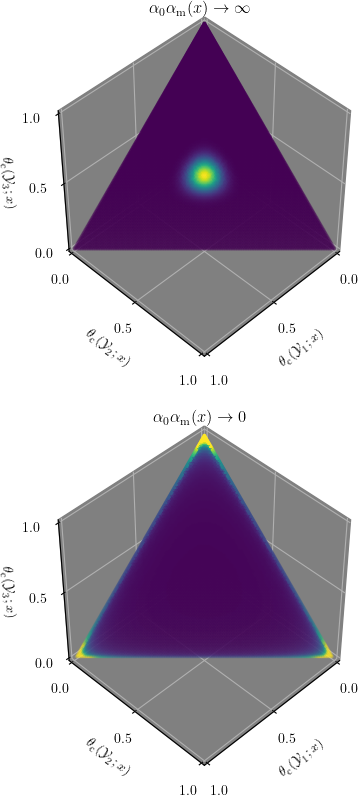
\includegraphics[width=0.65\linewidth]{SSP_2021/presentation/dir_loc.png}
%\caption{}
\end{figure}

\end{column}

\end{columns}

\footcitetext{ferguson}


\end{frame}


%\begin{frame}
%\frametitle{Dirichlet Prior}
%
%\begin{columns}[c]
%
%\begin{column}{.45\linewidth}
%
%The probability density function (PDF) of the model $\uptheta \in \Theta$ is Dirichlet:
%\begin{IEEEeqnarray*}{L}
%\prm_{\uptheta}(\theta) = \Dir\big( \theta ; \alpha \big) \\
%\quad = \beta(\alpha)^{-1} \prod_{y \in \Ycal} \prod_{x \in \Xcal} \theta(y,x)^{\alpha(y,x) - 1}
%\end{IEEEeqnarray*}
%
%\end{column}
%
%\hspace{2ex}
%\huge
%\begin{column}{.1\linewidth}
%$\Rightarrow$ \\ $\Rightarrow$
%\end{column}
%\normalsize
%\hspace{-3ex}
%
%\begin{column}{.45\linewidth}
%
%Conditional PDF of $\upthetac$ given $\upthetam$ is
%\begin{IEEEeqnarray*}{L}
%\prm_{\upthetac | \upthetam}\big( \thetac | \thetam \big) = \prm_{\upthetac}\big( \thetac \big) \\
%\quad= \prod_{x \in \Xcal} \Dir\Big( \thetac(x) ; \alpha(\cdot,x) \Big) \Big|_{\alpha(\cdot,x) = 1} \\
%\quad = \Big[ \big( |\Ycal|-1 \big)! \Big]^{|\Xcal|}
%\end{IEEEeqnarray*}
%
%\end{column}
%
%\end{columns}
%
%\vspace{1em}
%
%\vspace{1em}
%\centering
%\fcolorbox{NRL_blue}{NRL_blue}{\color{white}
%\parbox{37em}{
%\centering
%\large
%\textbf{True predictive distribution $\upthetac$ is independent \\of the marginal model and inherits a uniform PDF}
%}
%}
%\end{frame}








\begin{frame}
\frametitle{Model Posterior PDF}
\framesubtitle{Closed-Form}

\begin{itemize}
\item Independence of $\upthetac$ from $\upthetam$ implies conditional independence of $\upthetac$ from $\xrm$ given $\nbarrm$
\item As the data PMF $\Prm_{\nbarrm | \uptheta}$ has exponential form, the Dirichlet PDF is a conjugate prior 

\end{itemize}
\vspace{0.5em}
\begin{IEEEeqnarray*}{rCl}
\prm_{\upthetac | \xrm,\nbarrm}\big( \thetac | x,\bar{n} \big) & = & \prm_{\upthetac | \nbarrm}\big( \thetac | \bar{n} \big) \\
& = & \prod_{x' \in \Xcal} \Dir\Big( \thetac(x') ; \alpha(\cdot,x') \Big) \Big|_{\alpha(\cdot,x') = 1 + \bar{n}(\cdot,x')} \\
%= \prod_{x' \in \Xcal} \left[ \left( \sum_{y \in \Ycal} \bar{n}(y,x') + |\Ycal|-1 \right)! \prod_{y \in \Ycal} \frac{\thetac(y,x')^{\bar{n}(y,x')}}{\big(\sum_{y \in \Ycal} \bar{n}(y,x')\big)!} \right] 
\end{IEEEeqnarray*}

\vspace{0.5em}

\centering
\fcolorbox{NRL_blue}{NRL_blue}{\color{white}
\parbox{37em}{
\centering
\large
\textbf{Posterior for model $\upthetac(x)$ is Dirichlet and dependent \\solely on the sufficient statistic elements $\nbarrm(\cdot,x)$}
}
}

\end{frame}



\begin{frame}
\frametitle{Model Posterior PDF}
\framesubtitle{Asymptotic Trend}

\begin{columns}[T]

\begin{column}{.6\linewidth}

\begin{itemize}
\item Covariance of Dirichlet $\prm_{\upthetac(x) | \nbarrm(\cdot,x)}$ decreases monotonically with concentration $\alpha'(x) \equiv \sum_{y \in \Ycal} \alpha(y,x)$
\item Localized around $\mu_{\upthetac(x) | \nbarrm(\cdot,x)} = \alpha(\cdot,x)/\alpha'(x)$
\end{itemize}
\Large
\begin{equation*} 
\Downarrow \quad \Downarrow
\end{equation*}
\normalsize
As $n'(x) \equiv \sum_{y \in \Ycal} \bar{n}(y,x) \to \infty$, the posteriors converge to 
\begin{IEEEeqnarray*}{L}
\prm_{\upthetac(x) | \nbarrm(\cdot,x)}\Big(\thetac(x) | \bar{n}(\cdot,x) \Big) \to \delta\left( \thetac(x) - \frac{\bar{n}(\cdot,x)}{n'(x)} \right)
\end{IEEEeqnarray*}

\end{column}

\begin{column}{.4\linewidth}

\begin{figure}
\centering
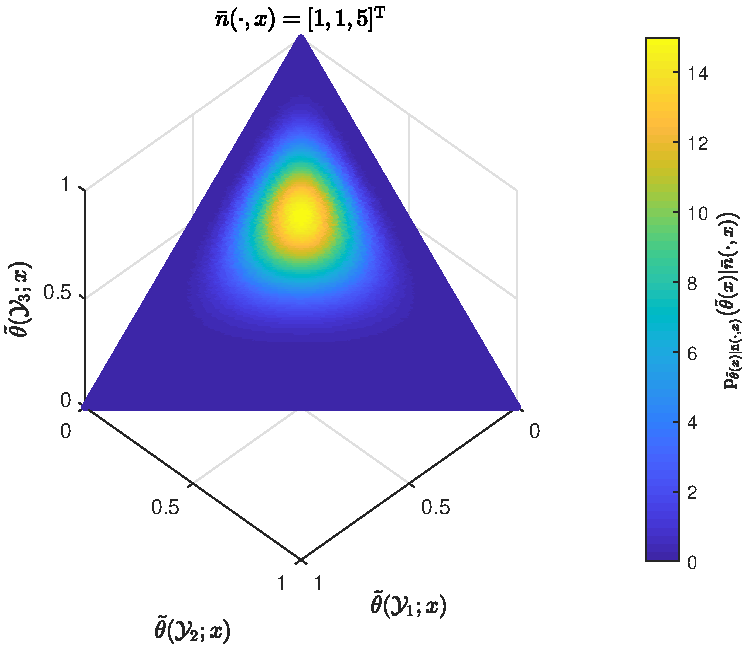
\includegraphics[width=0.9\linewidth]{P_theta_post_uni_tilde.pdf}
%\caption{}
\label{fig:P_theta_post_uni}
\end{figure}

\end{column}

\end{columns}

\vspace{1em}

\centering
\fcolorbox{NRL_blue}{NRL_blue}{\color{white}
\parbox{37em}{
\centering
\large
\textbf{Asymptotically consistent estimation of $\upthetac$ due to full support of prior}
}
}

\end{frame}




\begin{frame}
\frametitle{Bayesian Predictive PMF}

\textit{The Bayesian predictive PMF is a convex combination of two conditional distributions}:
\vspace{0.5em}
\begin{IEEEeqnarray*}{rCl} \label{P_y_xD_uniform}
\Prm_{\yrm | \xrm,\nbarrm}(\cdot | x,\bar{n}) & = & \mu_{\upthetac(x) | \nbarrm(\cdot,x)}\big( \bar{n}(\cdot,x) \big) \\
& \equiv & \left( \frac{|\Ycal|}{n'(x) + |\Ycal|} \right) \frac{1}{|\Ycal|} + \left( \frac{n'(x)}{n'(x) + |\Ycal|} \right) \frac{\bar{n}(\cdot,x)}{n'(x)} 
\end{IEEEeqnarray*}

\vspace{0.5em}

\begin{description}
\item[Prior Mean] Uniform PMF $\mu_{\upthetac(x)} = |\Ycal|^{-1}$ dependent only on the Dirichlet parameterization
\item[Conditional Empirical PMF] $\bar{n}(\cdot,x) / n'(x)$ dependent only on training data
\end{description}

\vspace{1em}

\centering
\fcolorbox{NRL_blue}{NRL_blue}{\color{white}
\parbox{37em}{
\centering
\large
\textbf{As the number of training data $n'(x)$ increases relative to the number of classes $|\Ycal|$, the predictive distribution tends toward the empirical PMF}
}
}

\end{frame}





\section{Bayesian Classifier and Error Trends}


\begin{frame}
\frametitle{Bayesian Classifier and Risk}

\textbf{Optimal Hypothesis}: the \emph{conditional majority decision}
\begin{IEEEeqnarray}{rCl} 
f^*(x;\bar{n}) & = & \argmax_{y \in \Ycal} \Prm_{\yrm | \xrm,\nbarrm}\big( y | x,\bar{n} \big) = \argmax_{y \in \Ycal} \bar{n}(y,x) \nonumber
\end{IEEEeqnarray}

\hrulefill
\vspace{0.5em}

\textbf{Minimum Expected Probability of Error}:
\begin{IEEEeqnarray*}{L}
\Rcal^* = 1 - \Erm_{\xrm,\Drm} \left[ \max_{y \in \Ycal} \Prm_{\yrm | \xrm,\Drm}(y | \xrm,\Drm) \right] = 1 - \sum_{x \in \Xcal} \frac{\Erm_{\nbarrm} \big[ \max_{y \in \Ycal} \bar{\nrm}(y,x) \big] + 1}{|\Ycal||\Xcal| + N} \nonumber \\
= 1 - \frac{\sum_{m=1}^{|\Ycal|} \binom{|\Ycal|}{m} (-1)^{m-1} \sum_{n=0}^{\big\lfloor\frac{N}{m}\big\rfloor} \prod_{l=1}^{|\Ycal||\Xcal|-1} \Big( 1-\frac{mn}{N+l} \Big)}{|\Ycal| + N/|\Xcal|} 
\end{IEEEeqnarray*}
\vspace{0.5em}
\begin{itemize}
\item[$*$] \emph{Efficient formula derived using Inclusion-Exclusion principle}
\end{itemize}

\end{frame}


\begin{frame}
\frametitle{Probability of Error Trends}
\framesubtitle{with Class/Data Set Sizes}

\begin{columns}[c]

\begin{column}{.5\linewidth}

\begin{figure}
\centering
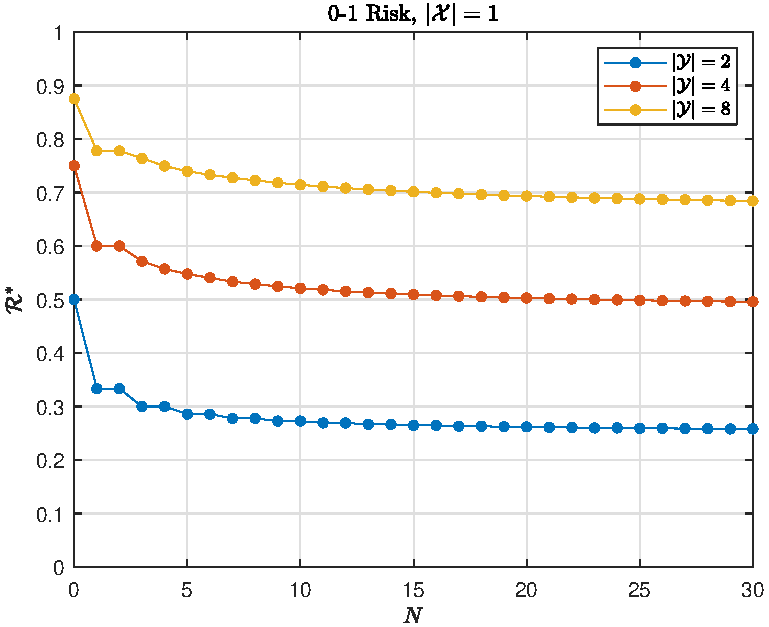
\includegraphics[width=0.8\linewidth]{Risk_01_uni_N_leg_My.pdf}
%\caption{Minimum 0--1 Risk for different numbers of classes}
\label{fig:Risk_01_uni_N_leg_My}
\end{figure}

\end{column}

\begin{column}{.5\linewidth}

\begin{figure}
\centering
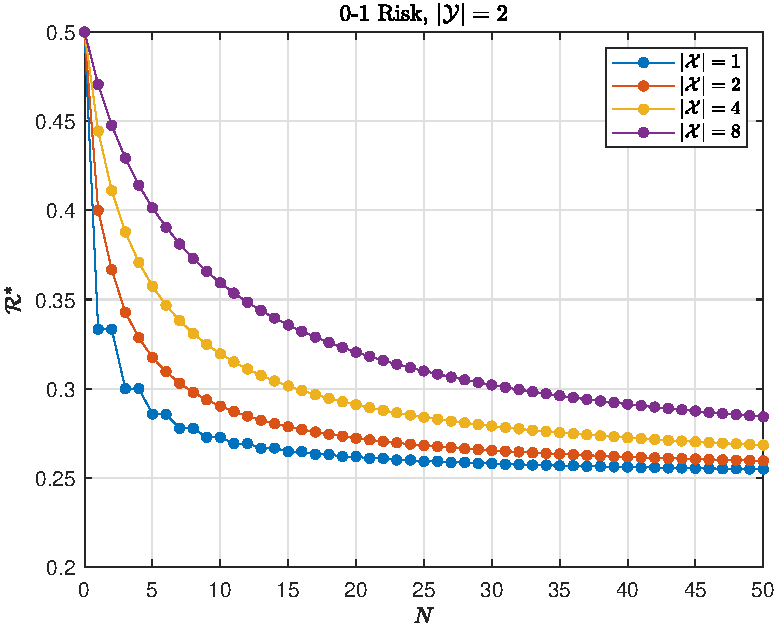
\includegraphics[width=0.8\linewidth]{Risk_01_uni_N_leg_Mx.pdf}
%\caption{Minimum 0--1 Risk for different numbers of possible observations}
\label{fig:Risk_01_uni_N_leg_Mx}
\end{figure}

\end{column}

\end{columns}

\begin{itemize}
\item Larger class sets $\Ycal$ raise the lower bound on probability of error
\item Larger observation set $\Xcal$ $\longrightarrow$ more data $N$ required to achieve the same level of performance
\end{itemize}

\end{frame}




\begin{frame}
\frametitle{Probability of Error Trends}
\framesubtitle{with Training Data Volume}

\begin{columns}[c]

\begin{column}{.5\linewidth}

\begin{itemize}
\item For binary classification, infinite training data only reduces the expected probability of error from 0.5 to 0.25
\item As $|\Ycal|$ increases, the probability of error tends to unity and any improvement due to training data becomes negligible
\end{itemize}

\begin{table}
\renewcommand{\arraystretch}{1.3}
\begin{tabular}{| c | c |}
\hline 
$N$ & $\Rcal^*$ \\
\hhline{|=|=|}
$0$ & $1 - |\Ycal|^{-1}$  \\ 
\hline
$\to \infty$ & $1 - |\Ycal|^{-1} \sum_{m=1}^{|\Ycal|} m^{-1}$ \\
\hline
\end{tabular}
%\caption{}
\end{table}

\end{column}

\begin{column}{.5\linewidth}

\begin{figure}
\centering
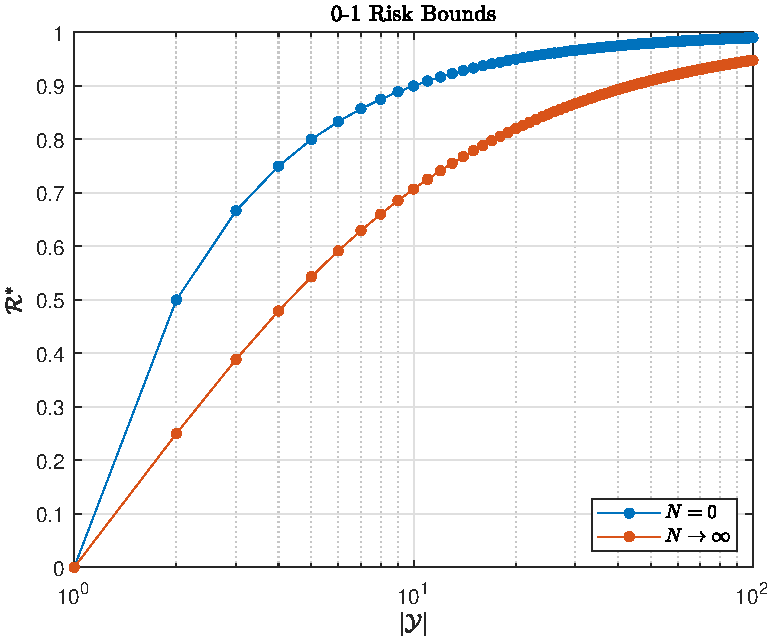
\includegraphics[width=1\linewidth]{Risk_01_uni_N_bounds.pdf}
%\caption{Minimum 0--1 Risk for zero and infinite number of training data}
\label{fig:Risk_01_uni_N_bounds}
\end{figure}

\end{column}

\end{columns}

\end{frame}


\begin{frame}
\frametitle{Comparison to Informative Classifiers}
\framesubtitle{Bayes Risk}

Classifiers derived from informative Dirichlet priors with $\alpha_f'(x) \gg |\Ycal||\Xcal|$ prioritize the prior mean $\mu_{\upthetac} = \alpha_f(\cdot,x) / \alpha_f'(x)$ for prediction

\vspace{-0.5em}
\begin{columns}[T]

\begin{column}{.5\linewidth}

\begin{figure}
\centering
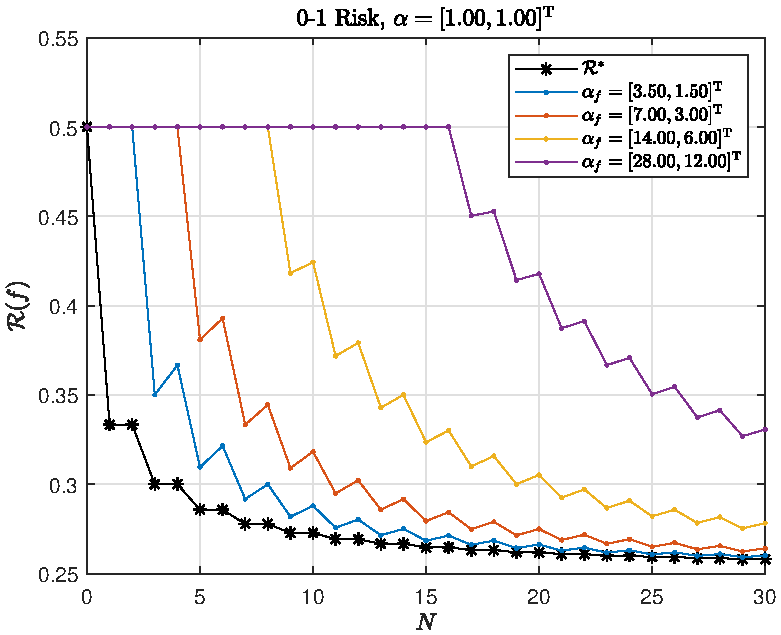
\includegraphics[width=0.8\linewidth]{Risk_01_Dir_N_leg_f_a0.pdf}
%\caption{}
\label{fig:Risk_01_Dir_N_leg_f_a0}
\end{figure}
\vspace{-2.5em}
\centering
\footnotesize
%Various $\alpha'(x)$

\end{column}

\begin{column}{.5\linewidth}

\begin{figure}
\centering
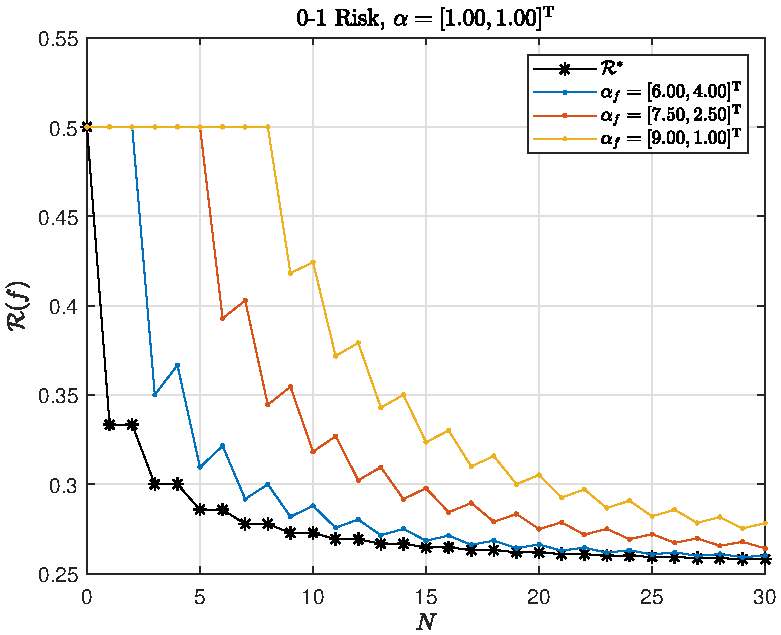
\includegraphics[width=0.8\linewidth]{Risk_01_Dir_N_leg_f_mu.pdf}
%\caption{}
\label{fig:Risk_01_Dir_N_leg_f_mu}
\end{figure}
\vspace{-2.5em}
\centering
\footnotesize
%Various $\mu_{\upthetac}$

\end{column}

\end{columns}

\vspace{1.8em}
\centering
\fcolorbox{NRL_blue}{NRL_blue}{\color{white}
\parbox{37em}{
\centering
\large
\textbf{Slower adaptation $\Rightarrow$ Higher Bayes probability of error}
}
}

\end{frame}



\begin{frame}
\frametitle{Comparison to Informative Classifiers}
\framesubtitle{Excess Conditional Risk}

\vspace{-1em}
\begin{columns}[c]

\begin{column}{.5\linewidth}

\begin{figure}
\centering
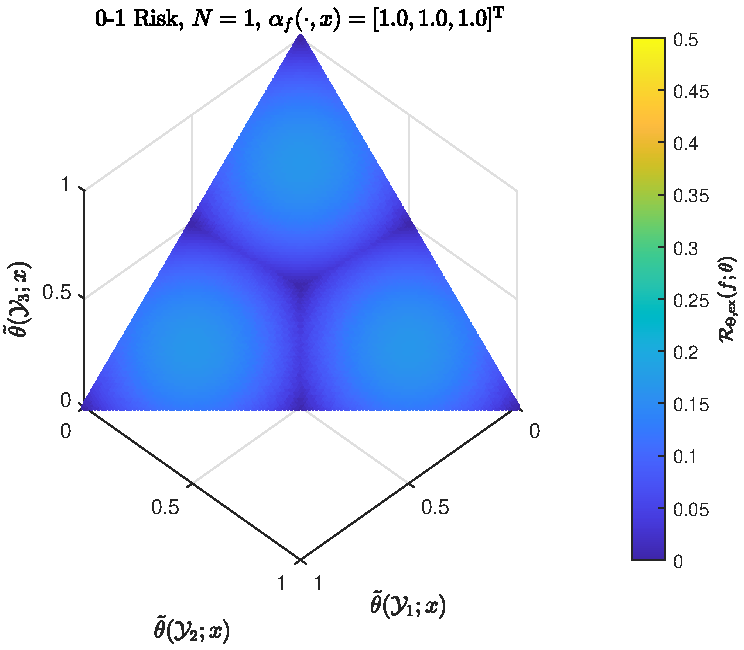
\includegraphics[width=0.8\linewidth]{Risk_cond_ex_01_Dir_theta__uni_clim.pdf}
%\caption{}
\label{fig:Risk_cond_ex_01_Dir_theta__uni}
\end{figure}

\end{column}

\begin{column}{.5\linewidth}

\begin{figure}
\centering
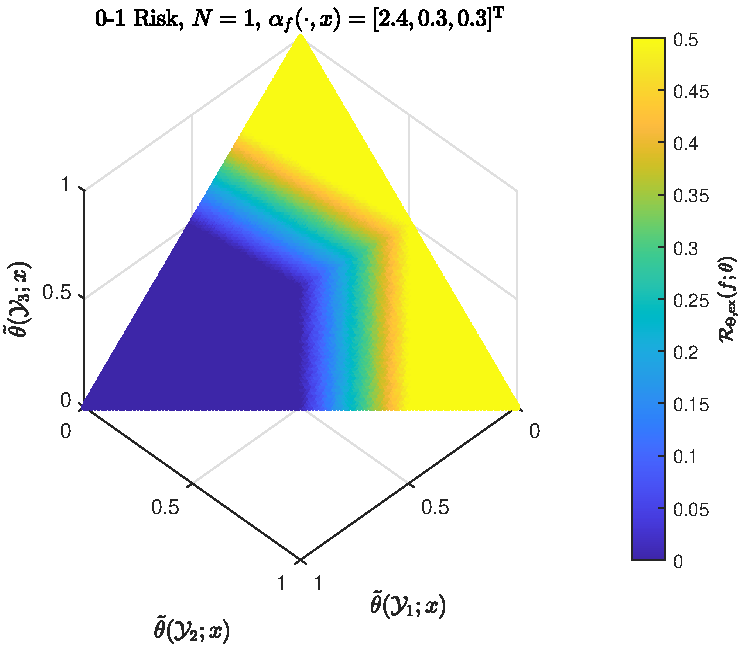
\includegraphics[width=0.8\linewidth]{Risk_cond_ex_01_Dir_theta__subj_clim.pdf}
%\caption{}
\label{fig:Risk_cond_ex_01_Dir_theta__subj}
\end{figure}

\end{column}

\end{columns}

\vspace{-0.2em}
\begin{block}{Trade-Off}
\textbf{Uniform prior provides a robust classifier for all unknown models $\theta$, limiting the space of high error models. However, fewer models achieve the clairvoyant risk.}
\end{block}


\end{frame}




\begin{frame}
\frametitle{Conclusions}

\begin{itemize}
\item The majority decision classifier designed with a uniform Dirichlet prior minimizes the possibility of maximal error for applications where the data distribution can not be adequately modeled
\item Full support of Dirichlet priors guarantees minimal risk in the limit of training data volume
\item Efficient closed-form for Bayesian probability of error provides a lower-bound for general classifiers
\end{itemize}

\begin{columns}[T]

\begin{column}{.55\linewidth}

\begin{itemize}
\item Low localization Dirichlet priors result in the same classifier - these priors are sensible for recognition applications where humans perform with low-error
\end{itemize}

\end{column}

\begin{column}{.4\linewidth}

\vspace{-2em}
\begin{figure}
\centering
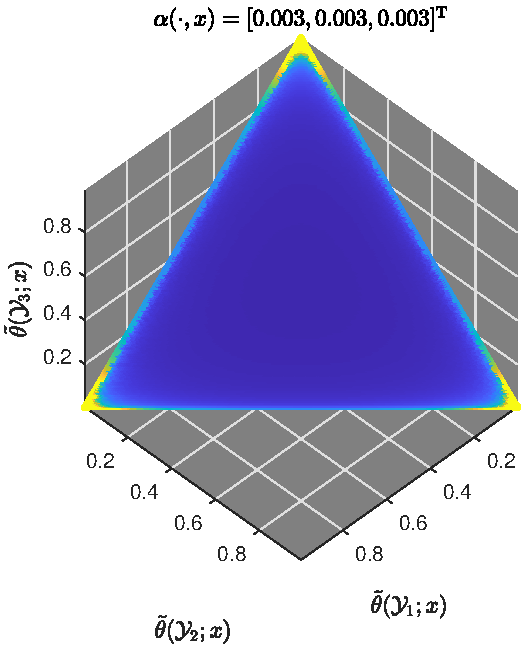
\includegraphics[width=0.5\linewidth]{P_theta_highVar.pdf}
%\caption{}
\label{fig:P_theta_highVar}
\end{figure}

\end{column}

\end{columns}


\end{frame}







\end{document}
